\subsection{Ablation}
\label{sec:ablation}
Table~\ref{tab:ablation} gives the contribution of each pipeline component.
Kernel ridge on loads and the reflection-averaged neural mean have test
errors \errKRRload\% and \errMLP\%, respectively. With a single mean,
stacking leaves the prediction unchanged; combining several means and
correcting their residuals both reduce error. The feature-space
and second input-space corrections did not improve validation error beyond the
first correction with a single mean and so were not selected.

Reflection test-time averaging lowers the metric-trained MLP's test error by
$\ttaGainMLP$ points. The reduction is consistent with Proposition~\ref{prop:sym}, whose exact
symmetry assumptions are stronger than the empirical agreement measured
in Supplement~\ref{sec:symcheck}. The effect is smaller on the
normalized-MSE network ($0.02$ points). Across the ten refiner seeds,
the implemented supplied-field average lowers test error by
$\ttaGainRefiner\pm\ttaGainRefinerSd$ percentage points (mean and sample standard deviation),
with an improvement at every seed. Random reflection augmentation during
training does not make the averaging effect vanish. The refiner's supplied-field operation and the full-map average are
distinguished in Supplement~\ref{sec:theory-sym}.
The kernel-flow regularizer did not improve
the low-data MLP's validation error. At high data, mean test errors without
reflection averaging are $\saKfMlpThree\%$ at weight $0.3$ and
$\saKfMlpZero\%$ without the regularizer, each over ten seeds. Weight $1.0$
gives $\saKfMlpOne\%$ over five seeds under the same scoring convention.

Replacing the single tuned Mat\'ern correction by a sum at several bandwidths
leaves validation error unchanged to two decimals under the stated search
and tuning budget. In the five-member experiment, nine seeds select the largest nugget
on the grid, $\lambda=10^{-3}$, and one selects $10^{-5}$. The length-scale
multiplier is $2$ at five seeds, $1$ at four and $4$ at one. The four-member
ablation selects multiplier $2$ at eight seeds.

The kernel prediction supplies the refiner's conditioning field. Its residual
is less correlated with the neural members' residuals on the measured splits,
which motivates this input. Section~\ref{sec:diversity} reports the
ensemble comparisons and their second-moment diagnostics.

\begin{table}[t]
\centering
\caption{Component contributions in the high-data pipeline. Mean relative $L^2$ test error under
the 20000-sample protocol; ``+'' rows are cumulative. All rows are mean $\pm$
standard deviation over ten seeds; the last two are the second experiment of
Section~\ref{sec:seeds}.}
\label{tab:ablation}
\begin{adjustbox}{max width=\linewidth}
\begin{tabular}{lc}
\toprule
Stage & Test error (\%) \\
\midrule
Kernel ridge on loads & $\errKRRload\pm\errKRRloadSd$ \\
Reflection-averaged neural mean & $\errMLP\pm\errMLPSd$ \\
\ \ + refiner and MSE variant, affine stack & $4.628\pm0.009$ \\
\ \ \ \ + residual kernel correction & $\errPipeFour\pm\errPipeFourSd$ \\
\ \ + FNO member, affine stack & $\errStack\pm\errStackSd$ \\
\ \ \ \ + residual kernel correction & $\errPipe\pm\errPipeSd$ \\
\ \ + complete FNO schedule and UNet member, affine stack & $\errSixStack\pm\errSixStackSd$ \\
\ \ \ \ + residual kernel correction & $\errSix\pm\errSixSd$ \\
\bottomrule
\end{tabular}
\end{adjustbox}
\end{table}


\subsection{Spatial structure of the residual error}
\label{sec:errors}

Ranked by relative error on the
validation split, the twenty hardest cases have error $\hardBest\%$ for the
reference member against a median of $\medRel\%$, a factor of $2.31$.
On those same cases the five-member ensemble reaches $\hardEns\%$ and the
mean over individual members is $\hardAll\%$. The ensemble improves this tail
only slightly. Because these cases were selected by the reference member's
errors, the comparison describes that selected subset.

The root-mean-square pointwise error over validation samples is $\rmsBnd$ on
the perimeter of the $41\times41$ grid and $\rmsInt$ in the interior, a ratio
of $1.59$; both vary across seeds by less than one percent of their values.
Averaging lowers them to $\rmsBndEns$ and $\rmsIntEns$. The concentration near
the loaded edge and supports remains visible in Figure~\ref{fig:fields}.
The shared spatial structure does not distinguish approximation bias from
numerical artifacts in the target fields.

\begin{figure}[t]
\centering
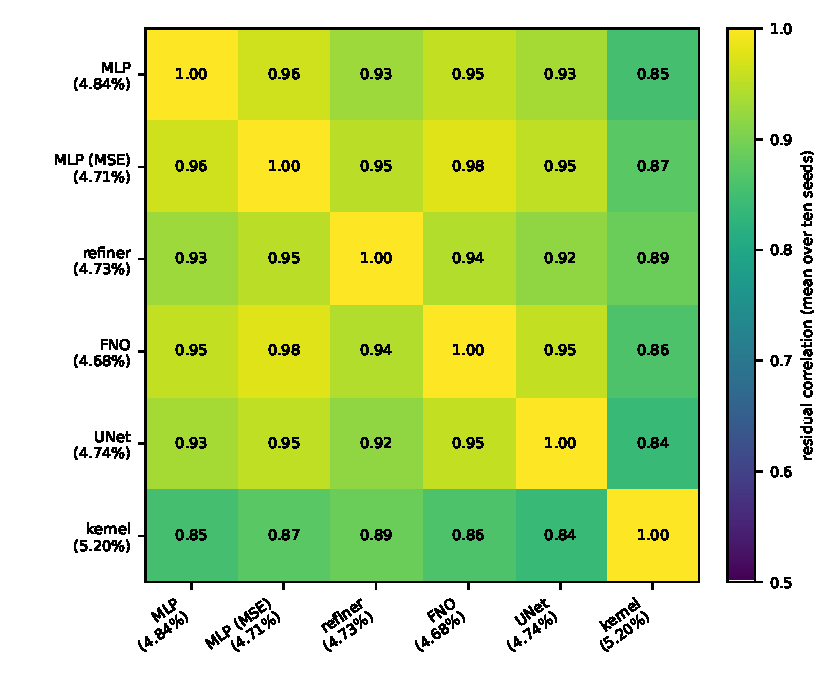
\includegraphics[width=0.62\linewidth]{figs/corr.pdf}
\caption{Centered correlation of per-sample normalized residuals on the validation
split, six members, averaged over the ten seeds of the second experiment.
Across seeds and pairs the entries range between $0.82$ and $0.98$.
The mean over pairs is $0.919\pm0.005$ across seeds; the kernel predictor
has correlation \corrKerLo--\corrKerHi{} with the normalized-MSE network
at every seed. These centered correlations differ from the uncentered
alignments summarized in Section~\ref{sec:diversity}.}
\label{fig:corr}
\end{figure}

\begin{figure}[t]
\centering
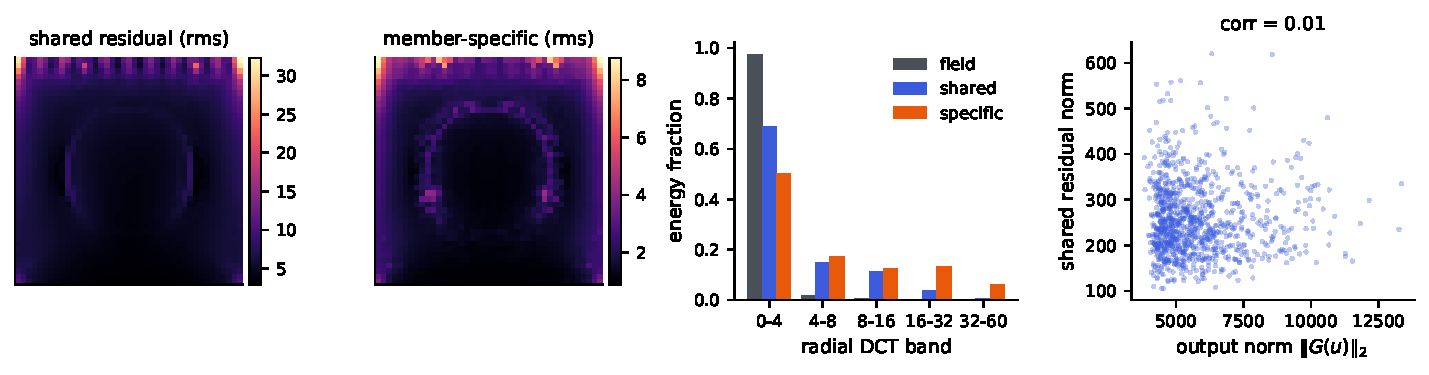
\includegraphics[width=\linewidth]{figs/shared.pdf}
\caption{Spatial and spectral structure of the shared residual $c$ (across-member mean of the
residual fields), at one seed. Left to right: rms of $c$ over the grid; rms of
the member-specific remainders; radial DCT band energies of the stress fields,
of $c$, and of the member-specific remainders; and the norm of $c$ against the output norm,
whose correlation is $0.01$.}
\label{fig:shared}
\end{figure}


\subsection{Spectra and effective dimension}
\label{sec:spectra}
A separate diagnostic uses $6000$ rows sampled
without replacement from the $19000$ training rows. The load coordinates are
standardized using the full training design. The Mat\'ern-$5/2$ length scale
is fixed at four times the median distance on a $2000$-row training subsample,
and the marked nugget is $10^{-5}$. These fixed diagnostic parameters need
not match those selected by each deployed correction. The split and sampling
generators both use seed~0.

The effective dimension is $d_{\mathrm{eff}}(10^{-5})=103.11885$,
where each eigenvalue $\mu_i$ contributes $\mu_i/(\mu_i+6000\lambda)$.
The Cholesky calculation of
$6000-6000\lambda\operatorname{tr}\big((K_S+6000\lambda I)^{-1}\big)$ agrees with the
eigenvalue sum to $1.7\times10^{-11}$. This calculation describes the
subsample smoother rather than the full $19000$-row fit. Low effective dimension does
not reduce the cubic work of the dense factorization used here.


\subsection{Computation and memory}
\label{sec:cost}
The structural-mechanics experiments use cloud CPU instances and dense,
exact linear solves for the kernel stages. At the experimental
dimensions, an eight-thread timing calculation measured $\costGramS$ seconds to
build a $19000\times19000$ Gram matrix in blocks, $\costCholS$ seconds for its
Cholesky factorization, and $\costSolveS$ seconds to solve for 1681 output
coordinates. The roughly one-minute total excludes hyperparameter search,
network training and prediction. Values in this timing experiment are
synthetic; the dimensions and operations match the experiment. The factorization
performs $n^3/3\approx2.3\times10^{12}$ floating-point operations. No GPU, inducing points, preconditioner or
stochastic linear solver is used in the correction.

Gram-matrix construction is the principal memory constraint at this size.
Forming a full squared-distance matrix and its
elementwise transforms allocates several $2.9$\,GB temporaries at once;
in the experiments this construction required more than the available
memory on a $31$\,GB instance. The block-filled timing
diagnostic has a measured peak of $\costPeakBlockGb$\,GiB, including the
factorization and solves, compared with $\costPeakNaiveGb$\,GiB after the
full-matrix construction. The reported pipeline uses full-size temporaries; the lower peak belongs
to the separate block-filled implementation. The neural means have a few million parameters and include both metric-loss
and normalized-MSE training. Splits are specified by permutation seeds and
inputs are the 41-dimensional loads described in Section~\ref{sec:benchmark}.

\subsection{Uncertainty quantification}
Theorem~\ref{thm:or} gives a conditional bound for a residual function in the
kernel native space with consistent training labels. The deployed correction
uses mixed training predictions: the kernel channel is constructed with
foldwise fits whose target centering uses the pooled training labels, while
neural predictions on these rows are in-sample. These labels need not equal
$G(X)-m_{\mathrm{full}}(X)$ for the deployed mean. The theorem applies to the deployed error under its stated consistency
and native-space assumptions and, where applicable, the mismatch term.

Table~\ref{tab:norms} reports a computable diagnostic: the squared RKHS norms
of ridge functions fitted to the two label arrays. With the selected
correction kernel at seed $0$, the residual-label fit has a norm about
\normRatio$\times$ smaller than the raw-stress fit and about
\normRatioNorm$\times$ smaller per unit label energy. These ratios depend on
the nugget and the scale. The mixed residual labels prevent identifying this
fitted norm with a lower bound for the native-space norm of the deployed
residual $G-m_{\mathrm{full}}$.

The design factor $P_\lambda$ correlates weakly with the deployed surrogate's
absolute error (Pearson \uqCorrAbs) and negatively with relative error. Its
correlation with the output norm is \uqCorrNorm{} (Figure~\ref{fig:uq}), so
its association with error depends on normalization by output amplitude.
Ensemble disagreement has correlation
$\uqDisAbs\pm0.006$ with absolute error across ten seeds and
$-0.25\pm0.04$ with relative error. The corresponding four-member absolute
error correlation is \uqDisAbsFour. Thus neither signal ranks the
remaining error well. A spread statistic is insensitive to a common additive
error shared by all members, which is consistent with the residual alignment
observed here.

Three bands are calibrated on $1000$ cases selected from the test block and
scored on the other $19000$: the scores are $\|e\|_2/P_\lambda$, $\|e\|_2$
(constant radius), and $\|e\|_2$ divided by ensemble disagreement. Each seed's
$P_\lambda$ uses its own selected correction kernel and training design.
The measured coverages are split diagnostics on the public test block. The marginal split-conformal theorem applies when the
predictor and score are fixed independently of exchangeable calibration and
future observations; the exact Beta and Beta--binomial descriptions additionally
require conditionally i.i.d. continuous scores (or an appropriate randomized
rank construction). A random partition of a fixed benchmark pool alone does not supply these
sampling assumptions.

For the six-member pipeline the $P_\lambda$ band has empirical coverage
$\uqPlamSix\pm\uqPlamSixSd\%$ at the nominal \uqCoverNom\% level and
$\uqPlamSixHi\pm\uqPlamSixHiSd\%$ at $95\%$. Under the i.i.d.-continuous
reference model, $m=1000$ gives latent coverage
$\mathrm{Beta}(901,100)$ at the $90\%$ level; with $19000$ independent
evaluation scores its central $95\%$ Beta--binomial reference interval is
$[88.0\%,91.8\%]$. At nominal $95\%$ coverage, the corresponding central
$95\%$ reference interval is $[93.5\%,96.3\%]$.
All ten six-member coverages fall inside these intervals at each
level.

The constant-radius band covers $\uqRawSix\pm\uqRawSixSd\%$ and
$\uqRawSixHi\pm\uqRawSixHiSd\%$, inside the reference intervals at ten of
ten seeds at both levels; the $P_\lambda$ band is on average
\uqWidthRatio{} times as wide. The disagreement-scaled band covers
$\uqDisSix\pm\uqDisSixSd\%$ and $\uqDisSixHi\pm\uqDisSixHiSd\%$, with
one seed on the upper edge of the $95\%$ reference interval. The five-member
pipeline gives $\uqPlamFive\pm\uqPlamFiveSd\%$ and
$\uqPlamFiveHi\pm\uqPlamFiveHiSd\%$ for the $P_\lambda$ band (ten and nine
seeds inside), and $\uqRawFive\pm\uqRawFiveSd\%$ and
$\uqRawFiveHi\pm\uqRawFiveHiSd\%$ for the constant-radius band (ten inside
at both levels). The constant-radius band is narrower, and the kernel design factor
provides no measured efficiency gain.

\begin{table}[t]
\centering
\caption{Fitted-norm diagnostic of the residual correction at seed $0$ of the
complete-schedule experiment: the same validated correction kernel (scale
multiplier $2$, nugget $10^{-3}$, median length scale) ridge-fitted to the
raw stress fields and to the six-member stack residuals on the training
split. $\|\widehat r\|_K^2=\operatorname{tr}(\alpha^\top K\alpha)$ is the
squared RKHS norm of the fitted function; the last column divides it by
the energy of the fitted label array. The residual labels mix foldwise
kernel predictions and in-sample neural predictions, so these numbers are
not identified as lower bounds for the native-space norm of the deployed
residual. The ratios depend on the selected nugget and scale. Much of the raw
ratio reflects output amplitude: per unit energy the
residual's fitted norm is \normRatioNorm{} times smaller at this seed, not
\normRatio{}; at seeds $1$ and $2$, whose corrections chose scale
multipliers $1$ and $2$, the raw ratios are \normRatioLo{} and $4300$ and the
normalized ones \normRatioNormLo{} and $7.6$. }
\label{tab:norms}
\begin{adjustbox}{max width=\linewidth}
\begin{tabular}{lccc}
\toprule
Kernel regresses & $\|\widehat r\|_K^2$ & energy $\|T\|_F^2$ & $\|\widehat r\|_K^2/\|T\|_F^2$ \\
\midrule
Raw stress fields ($m=0$) & $7.12\times10^{8}$ & $6.77\times10^{11}$ & $1.05\times10^{-3}$ \\
Ensemble residuals & $1.45\times10^{5}$ & $1.21\times10^{9}$ & $1.20\times10^{-4}$ \\
\midrule
Ratio & \normRatio$\times$ & \normEnergyRatio$\times$ & \normRatioNorm$\times$ \\
\bottomrule
\end{tabular}
\end{adjustbox}
\end{table}

\begin{figure}[t]
\centering
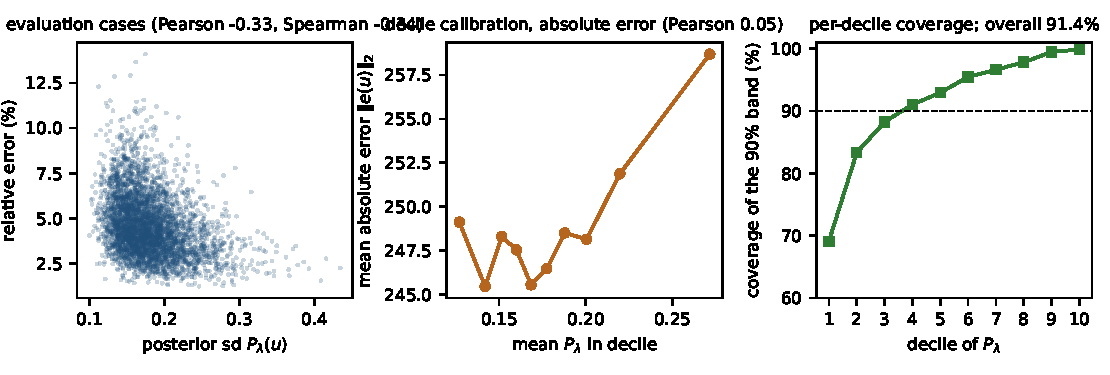
\includegraphics[width=\linewidth]{figs/uq.pdf}
\caption{Uncertainty measures for the six-member correction at seed 0.
Calibration uses $1000$ test-block cases and evaluation uses the other
$19000$, as in Section~\ref{sec:uq}. Left: the Gaussian process
posterior standard deviation $P_\lambda$ against relative error; the
association is negative (Pearson $-0.33$) because large-amplitude outputs have
small relative error. Middle: decile calibration of $P_\lambda$ against
absolute error $\|e(u)\|_2$; the
association is weak (Pearson $0.05$). Right: coverage of the
$P_\lambda$-scaled $90\%$ band within each decile of $P_\lambda$: $91.4\%$
overall, but from $69\%$ in the lowest decile to $99.9\%$ in the highest,
so coverage varies strongly with the design factor despite an overall
value close to the nominal level. Across the ten seeds the same band
has coverage $\uqPlamSix\pm\uqPlamSixSd\%$ at the nominal \uqCoverNom\% level,
inside the i.i.d.-continuous Beta--binomial reference interval at ten
seeds of ten; the constant-radius band
is the narrower of the two (Section~\ref{sec:uq}).}
\label{fig:uq}
\end{figure}

\begin{figure}[t]
\centering
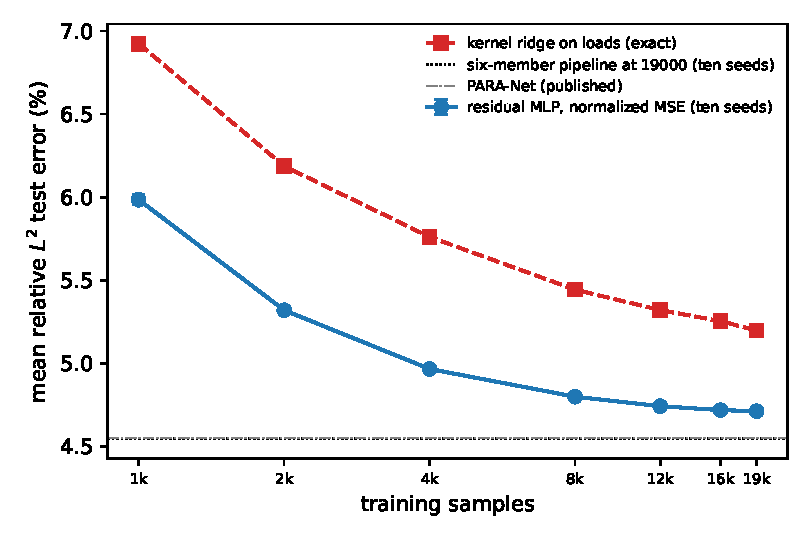
\includegraphics[width=\linewidth]{figs/curve_seeded.pdf}
\caption{Structural-mechanics learning curves. The first
$N+1000$ rows of the training pool are used, with the final $1000$ reserved
for validation and the first $N$ for fitting. The validation split is fixed
across seeds at each $N$ and changes with $N$; evaluation uses the full test
block. The curves give mean relative test error for the normalized-MSE
network (mean and standard deviation over ten seeds) and deterministic
Mat\'ern kernel ridge on loads, with both axes logarithmic. The horizontal lines mark the six-member pipeline at $19000$
samples and the quoted PARA-Net result. Error bars are smaller than the
markers above $4000$.}
\label{fig:scaling}
\end{figure}


\subsection{Seed variation and test-sample uncertainty}

The seed standard deviations describe variation from initialization and
selection on a common fixed test block. They do not include the
sampling uncertainty of a future evaluation set. If cases were independent
and representative of a target population, the reported per-case standard
deviation $0.0169$ would give a mean-error standard error of $\seTest$
percentage points over $20000$ cases.

The published baselines do not provide per-case predictions or comparable
training replicates. Their differences from our scores therefore do not
support a paired significance test or an equivalence conclusion. Combining
two copies of our sampling term in quadrature gives approximately
$\seUnpaired$ points, but this imputes an unknown baseline variance and
covariance structure. It is a sensitivity calculation. The $0.098$-point difference from PCA-Net
and $0.022$-point difference from PARA-Net for the five-member pipeline are
benchmark-score differences whose statistical uncertainty cannot be
determined from the available baseline summaries.

Within the two experiments, per-case paired differences isolate changes
between fitted predictors on the same cases. The full pipeline reduces error by
$\errEndToEnd$ percentage points, and removing the FNO increases it by
$\fnoGain\pm\fnoGainSd$ points across ten seeds, with the latter direction
holding at all ten.

The validation second-moment simplex optimum distributes weight among the
five members: refiner $0.31\pm0.04$, FNO $0.34\pm0.06$, normalized-MSE network
$0.24\pm0.08$, kernel $0.06\pm0.03$, and metric-trained MLP $0.06\pm0.04$.
The kernel has nonzero weight at all ten seeds and the metric-trained MLP at
nine. For the six-member experiment the corresponding shares are UNet
$0.32\pm0.06$, FNO $0.30\pm0.07$, refiner $0.27\pm0.04$, kernel
$0.06\pm0.02$, normalized-MSE network $0.03\pm0.04$, and metric-trained MLP
$0.02\pm0.02$. The FNO's large share despite its single-member ranking
illustrates the role of off-diagonal residual second moments.

Proposition~\ref{prop:secmom}(i) uses the uncentered alignment
$S_{12}/\sqrt{S_{11}S_{22}}$. The descriptive centered correlations in
Figure~\ref{fig:corr} need not equal this alignment. Exact convex-mixture
calculations use the uncentered second-moment matrix, rather than the
centered-correlation summaries.

The completed FNO schedule reduces its validation RMS error from $\fnoRmsA\%$ to
$\fnoRmsB\%$, while its descriptive correlation with the normalized-MSE
network increases from $\corrFnoLo$--$\corrFnoHi$ to $0.974$--$0.980$.
The five-member validation quadratic optimum is $\predRMS\%$ before
and $\predRMSFiveC\%$ after this change. These measured changes are consistent with an accuracy
improvement being offset by greater residual alignment.
Proposition~\ref{prop:exchange} gives a local sensitivity calculation for
fixed positive RMS errors and uncentered alignment; the centered-correlation
summaries do not determine that sensitivity.

For an exactly equicorrelated equal-error family,
Proposition~\ref{prop:secmom}(ii) gives the limiting RMS value
$\bar e\sqrt{\bar\varrho}$. Substituting the measured mean RMS error gives
the heuristic value $\ensFloor\pm\ensFloorSd\%$ for five members using
the mean centered correlation, and $\ensFloorSix\pm\ensFloorSixSd\%$
for six members using the mean uncentered alignment. The empirical pools are heterogeneous,
so these substitutions are heuristic diagnostics. The
one-sided entrywise bounds below and the sixty-member bound use the actual
uncentered second-moment matrices instead.

All these bounds concern RMS error $\mathcal E_2$ for global convex weights.
Jensen's inequality gives $\mathcal E_1\le\mathcal E_2$ for the same
predictor, so an RMS lower bound does not transfer to mean error. The deployed
pipeline's per-pixel affine weights and kernel correction also place it
outside the global convex class. Among global sum-to-one weights the signed
and convex optima differ by at most $0.00052$ percentage points across the fitted pools, but they do not always coincide: the signed minimizer has a negative
coordinate at seven six-member seeds and one five-member seed.

The selected input-space residual correction improves the five-member stack
by $\corrGain$ points at $n=19000$. Figure~\ref{fig:scaling}
reports the observed response to sample size: the normalized-MSE network
goes from $\lcMlpOneK\pm\lcMlpOneKSd\%$ at $N=1000$ to
$\lcMlpEightK\pm\lcMlpEightKSd\%$ at $8000$ and
$\lcMlpNineteenK\pm\lcMlpNineteenKSd\%$ at $19000$; the kernel goes from
$\lcKrrOneK\%$ to $\lcKrrEightK\%$ and $\lcKrrNineteenK\%$.
Over the measured range above $8000$, fitted log-log slopes are
$-\lcSlopeMlp\pm\lcSlopeMlpSd$ for the network and $-\lcSlopeKrr$ for the
kernel. The final increase in sample size reduces error by
$\lcLastGain\pm\lcLastGainSd$ percentage points, with a reduction at
nine seeds. The last two increases together reduce error by
$\lcLastTwoGain\pm\lcLastTwoGainSd$ percentage points, with a reduction
at all ten seeds. These are finite-range fits.
A three-parameter fit $e_\infty+cN^{-\alpha}$ gives different extrapolated
asymptotes, $4.64\%$ and $4.88\%$, so it does not locate a common floor.
Shared
approximation bias and target discretization artifacts remain unresolved
explanations for the residual plateau.

On the five-member test set, Corollary~\ref{cor:floorpinch} gives a
normalized bracket $[0.949\pm0.005,1.039\pm0.004]$ and fitted-global-stack
quadratic risk $0.980\pm0.003$. That risk uses the deployed global weights. The six-member validation-matrix
calculation reports a bracket $[0.933\pm0.007,1.032\pm0.004]$ and normalized
simplex optimum $0.972\pm0.005$. The corollary upper-bounds the minimum by
the uniform-weight risk; an arbitrary fitted ensemble need not lie below
that upper bound, although the five-member weights do.

From the six-member validation matrices, the one-sided
RMS floor $\sqrt{\min_{i\ne j}S_{ij}}$ is $4.820\pm0.062\%$, the stronger
finite-six-member lower bound is $4.849\pm0.060\%$, and the quadratic
optimum is $\predRMSSix\pm\predRMSSixSd\%$. The dispersion factors
$\dispFac\pm\dispFacSd$ and $\dispFacSix\pm\dispFacSixSd$ compare
$\mathcal E_1$ and $\mathcal E_2$ on the same validation data used to compute
the weights. They measure the difference between the two metrics on those validation data. For six members the ratio of test mean error to validation RMS
error is $0.9357\pm0.0110$; that ratio additionally includes transfer between
samples and is not a pure dispersion factor.

\paragraph{The sixty-predictor pool.} The analysis of
Section~\ref{sec:seeds-arch} uses the test predictions of all sixty
members in the second experiment. A fixed permutation divides
the test block into $1000$ fitting and $19000$ evaluation cases for this
pooling exercise. Convex weights fitted on the first subset
are evaluated on the second; the hindsight optimum is explicitly optimized
on the evaluation matrix. Equal-weight seed curves average over all subsets
for RMS error; mean errors use all subsets where there are at most $45$, and
$40$ random subsets otherwise.

Using the evaluation matrix, the smallest diagonal is $0.0024512070$ and the
within- and between-architecture lower second moments divided by that
diagonal are $0.9807963$ and $0.9377968$. Theorem~\ref{thm:blockfloor} then
gives $\saBound\%$, below the hindsight RMS optimum
$\saSixtyOracleRms\%$. This empirical lower bound applies to global convex combinations of these
sixty predictors on the evaluation cases.
An extension to more seeds would require the same entrywise lower bounds to
hold for those additional members.

Within the existing ten-seed blocks, square roots of the smallest
within-architecture second moments are approximately $4.93\%$ for the FNO,
$4.96\%$ for the normalized-MSE network, $4.97\%$ for the refiner,
$4.94\%$ for the UNet, $4.90\%$ for the metric-loss MLP and $5.46\%$ for
the kernel. The corresponding ten-seed equal-weight errors lie close to
these empirical references. Replacing lower moments by mean moments in the block formula
returns the uniform sixty-member mixture's value exactly, as an algebraic identity.

At the pipeline's fixed ridge, per-pixel affine fitting on all sixty members
has evaluation error $\saPerpixSixty\%$, versus $\saPerpixMeans\%$ for the
six ten-seed means and $\saPerpixSeedZero\%$ for six members at seed~0.
The leave-one-out ridge comparisons in Section~\ref{sec:seeds-arch} show that
this difference depends on regularization. Removing the UNet seeds changes the
uniform-weight mean error from $\saSixtyEq\%$ to $\saFiftyEq\%$.

For the first experiment the test-error seed standard deviation is $0.005$
points at uniform weights, $0.006$ for fitted global weights,
$\errStackSd$ for the affine stack and $\errPipeSd$ after correction.

\begin{figure}[t]
\centering
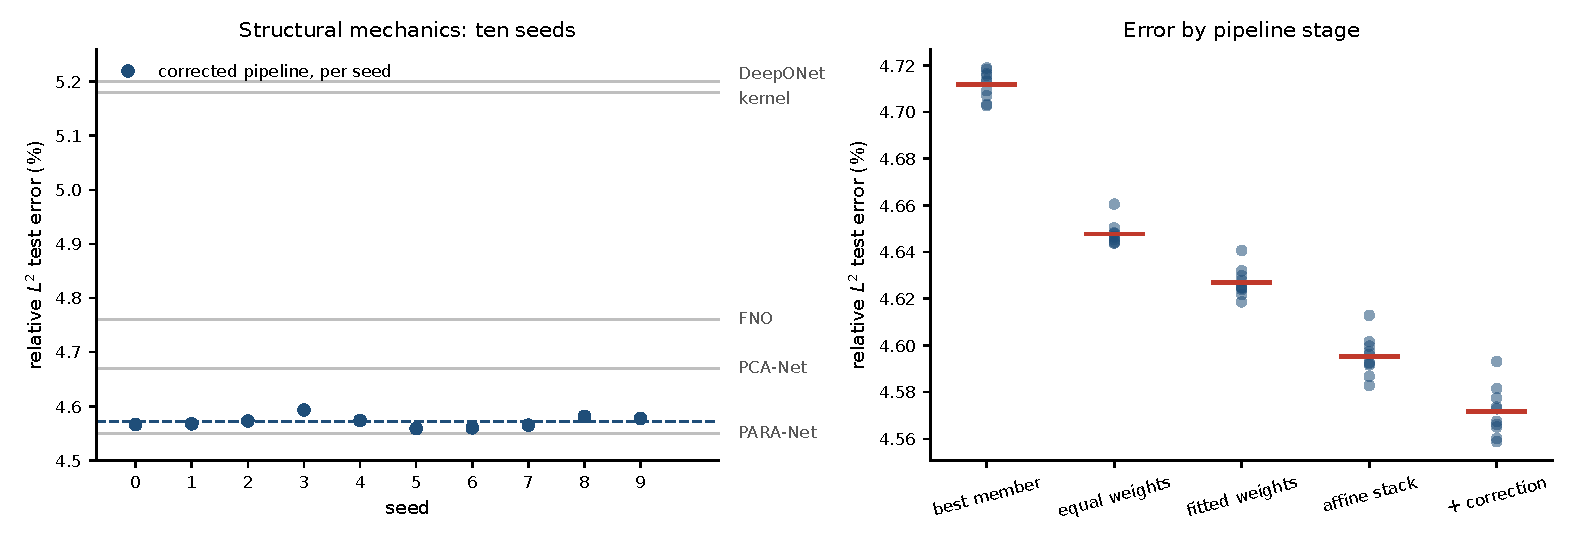
\includegraphics[width=\linewidth]{figs/seedspread.pdf}
\caption{Left: the corrected pipeline's test error at each of the ten seeds
(points), their mean (dashed), and the five published benchmark errors on the
same axis (grey). These show the variability of our pipeline;
comparable seed distributions are unavailable for the published methods. Right: test error at successive pipeline stages for each seed, with the
stage means marked. Fitting per-pixel weights lowers the
mean; seed spreads at each stage are reported in the text.}
\label{fig:seedspread}
\end{figure}
